\section{Prediction for unassociated sources in 3FGL and comparison with 4FGL}
\lb{sec:3FGLprediction}


In this section we describe the use of the best algorithms from the previous section to predict classes for the unassociated sources in the 3FGL. We then use the associations which exist for some of these sources in the 4FGL to check the accuracy of our methods on the unassociated data.  A total of 286 such sources were identified. These contain 20 Pulsars. \\


\subsection{3FGL Unassociated sources with Association in 4FGL}
There were a total of 286 sources without associations in 3FGL but which had a corresponding assocation in 4FGL. We trained our algorithms on the entire set of associated data from the 3FGL, and then tested our algorithms on these 286 sources. The probabilistic version is discussed in the next section.  \\

Here we can see how Random Forests and BDT accuracies depend on the complexity of the network. Random Forests follow the same pattern as seen with the associated data with greater complexity allowing for a higher accuracy of the sources. Boosted Decision Trees also lower the accuracy as the maximum depth increases, although there seem to be certain points where the accuracy suddenly rises up. As seen with the training data, here also the BDT models converge to an accuracy value which is only dependent on the number of trees\\

\begin{figure}[h]
%\centerin
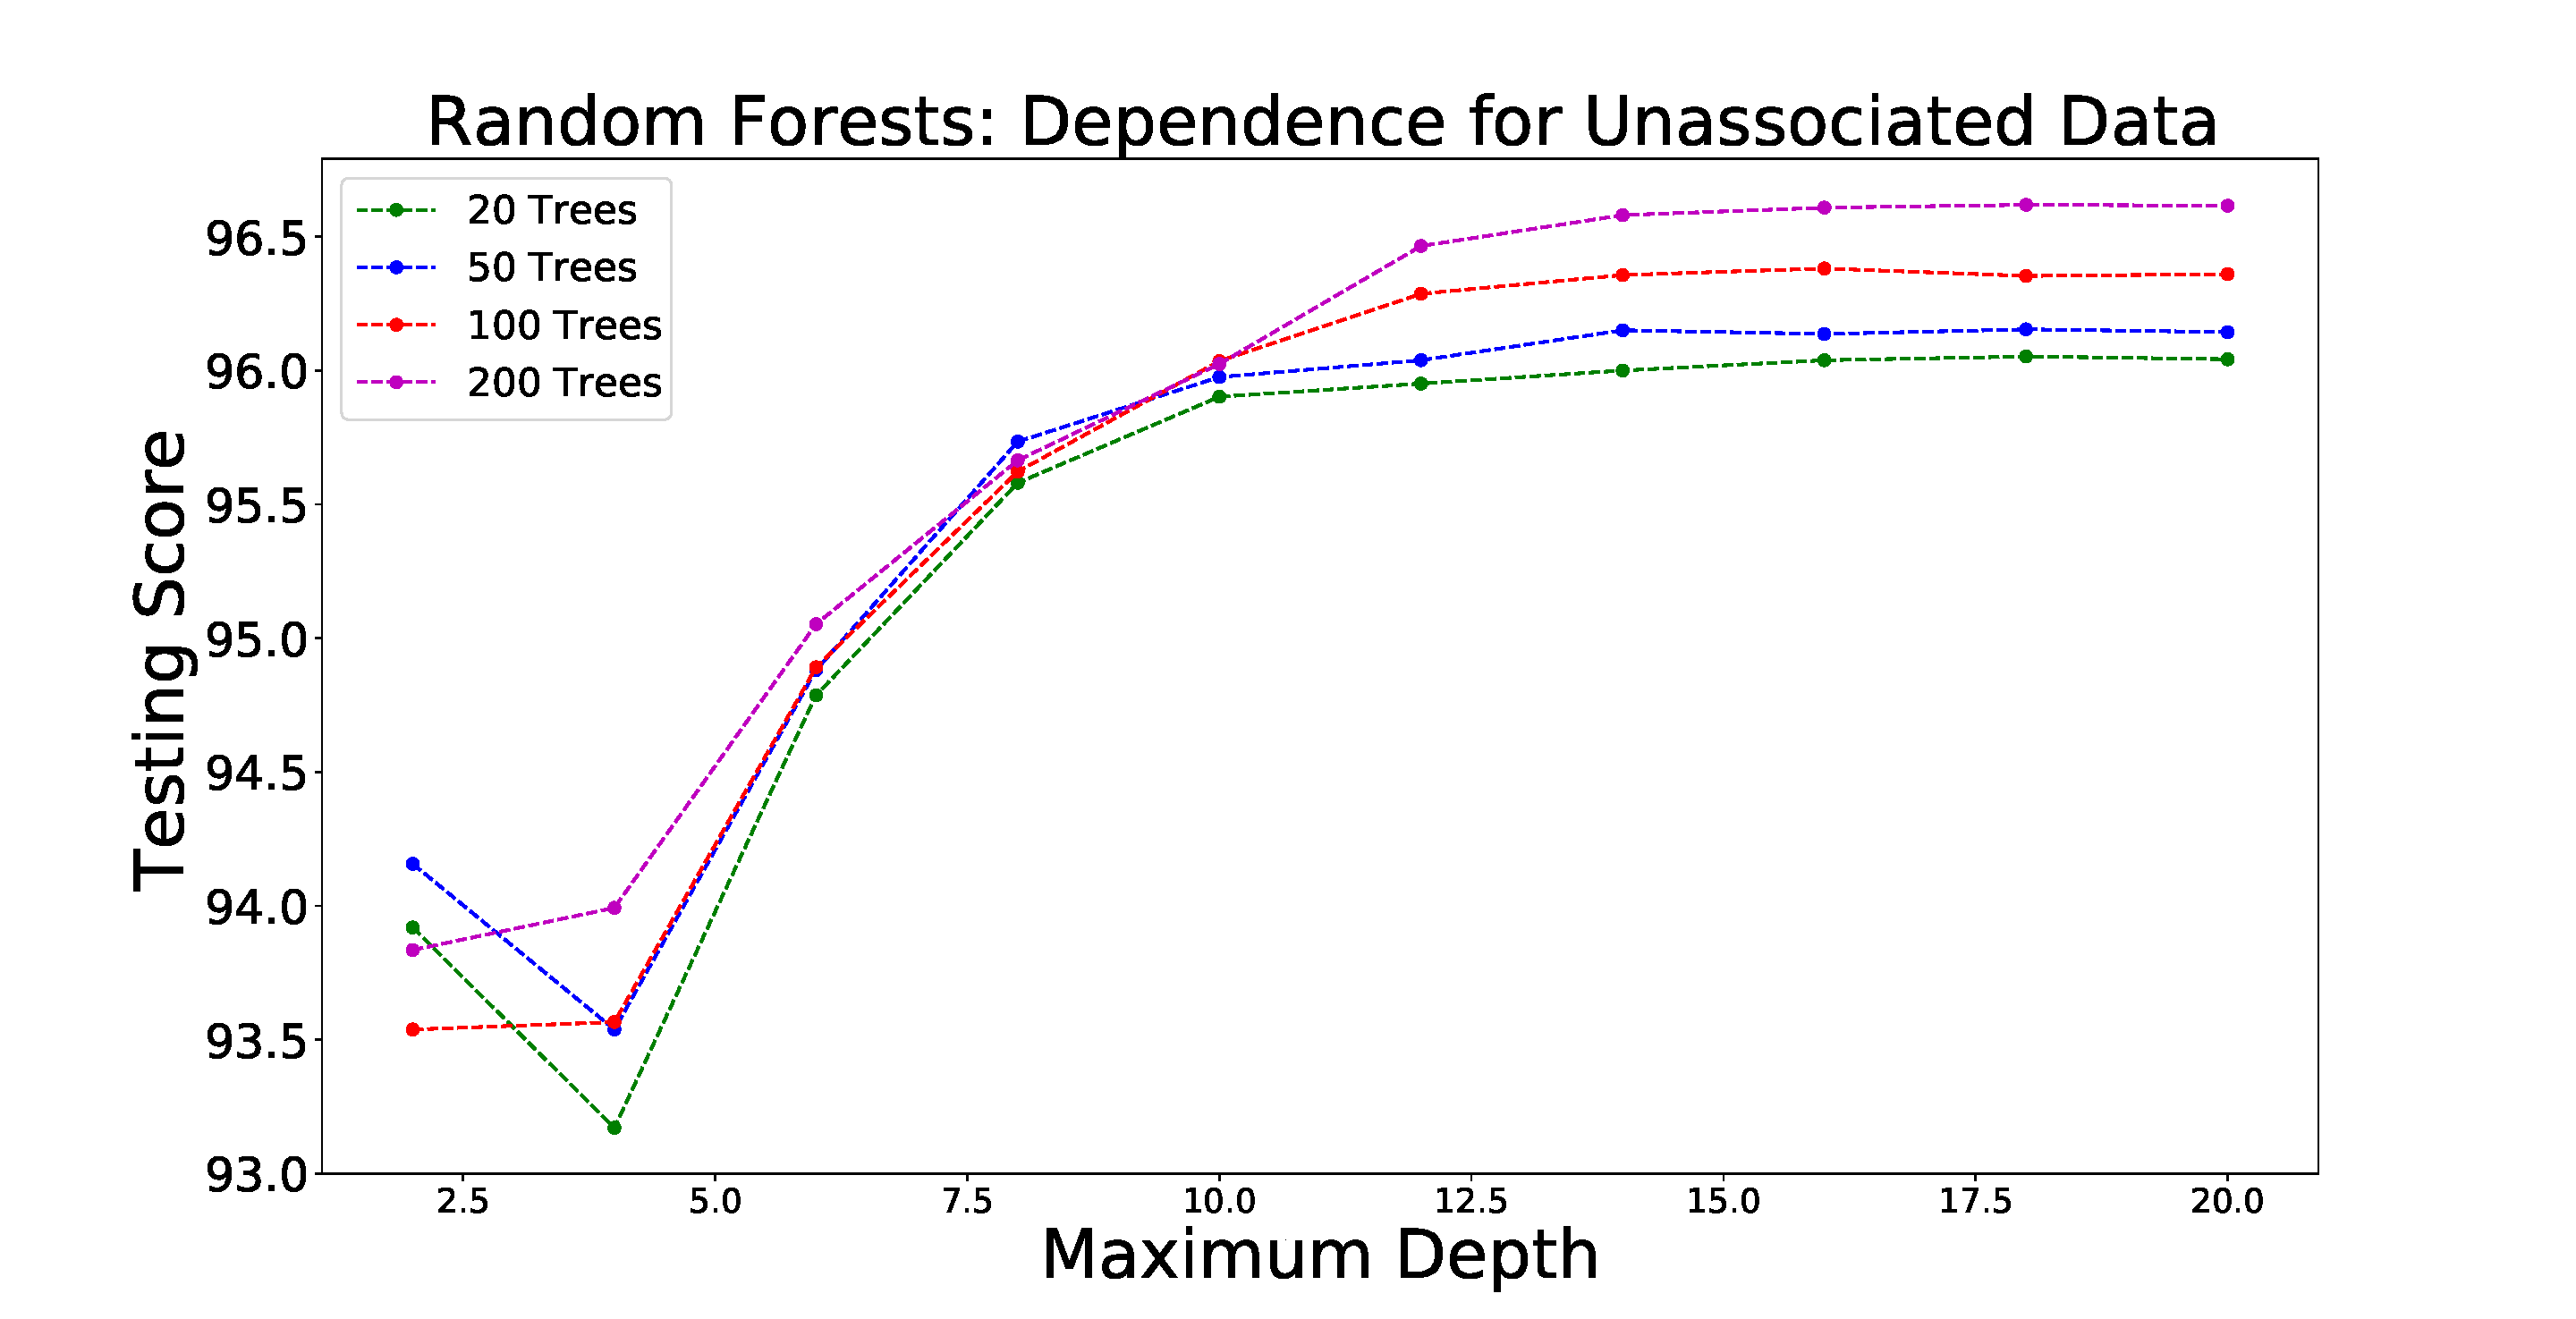
\includegraphics[width=\twopicsp\textwidth]{plots/unassoc2.pdf}
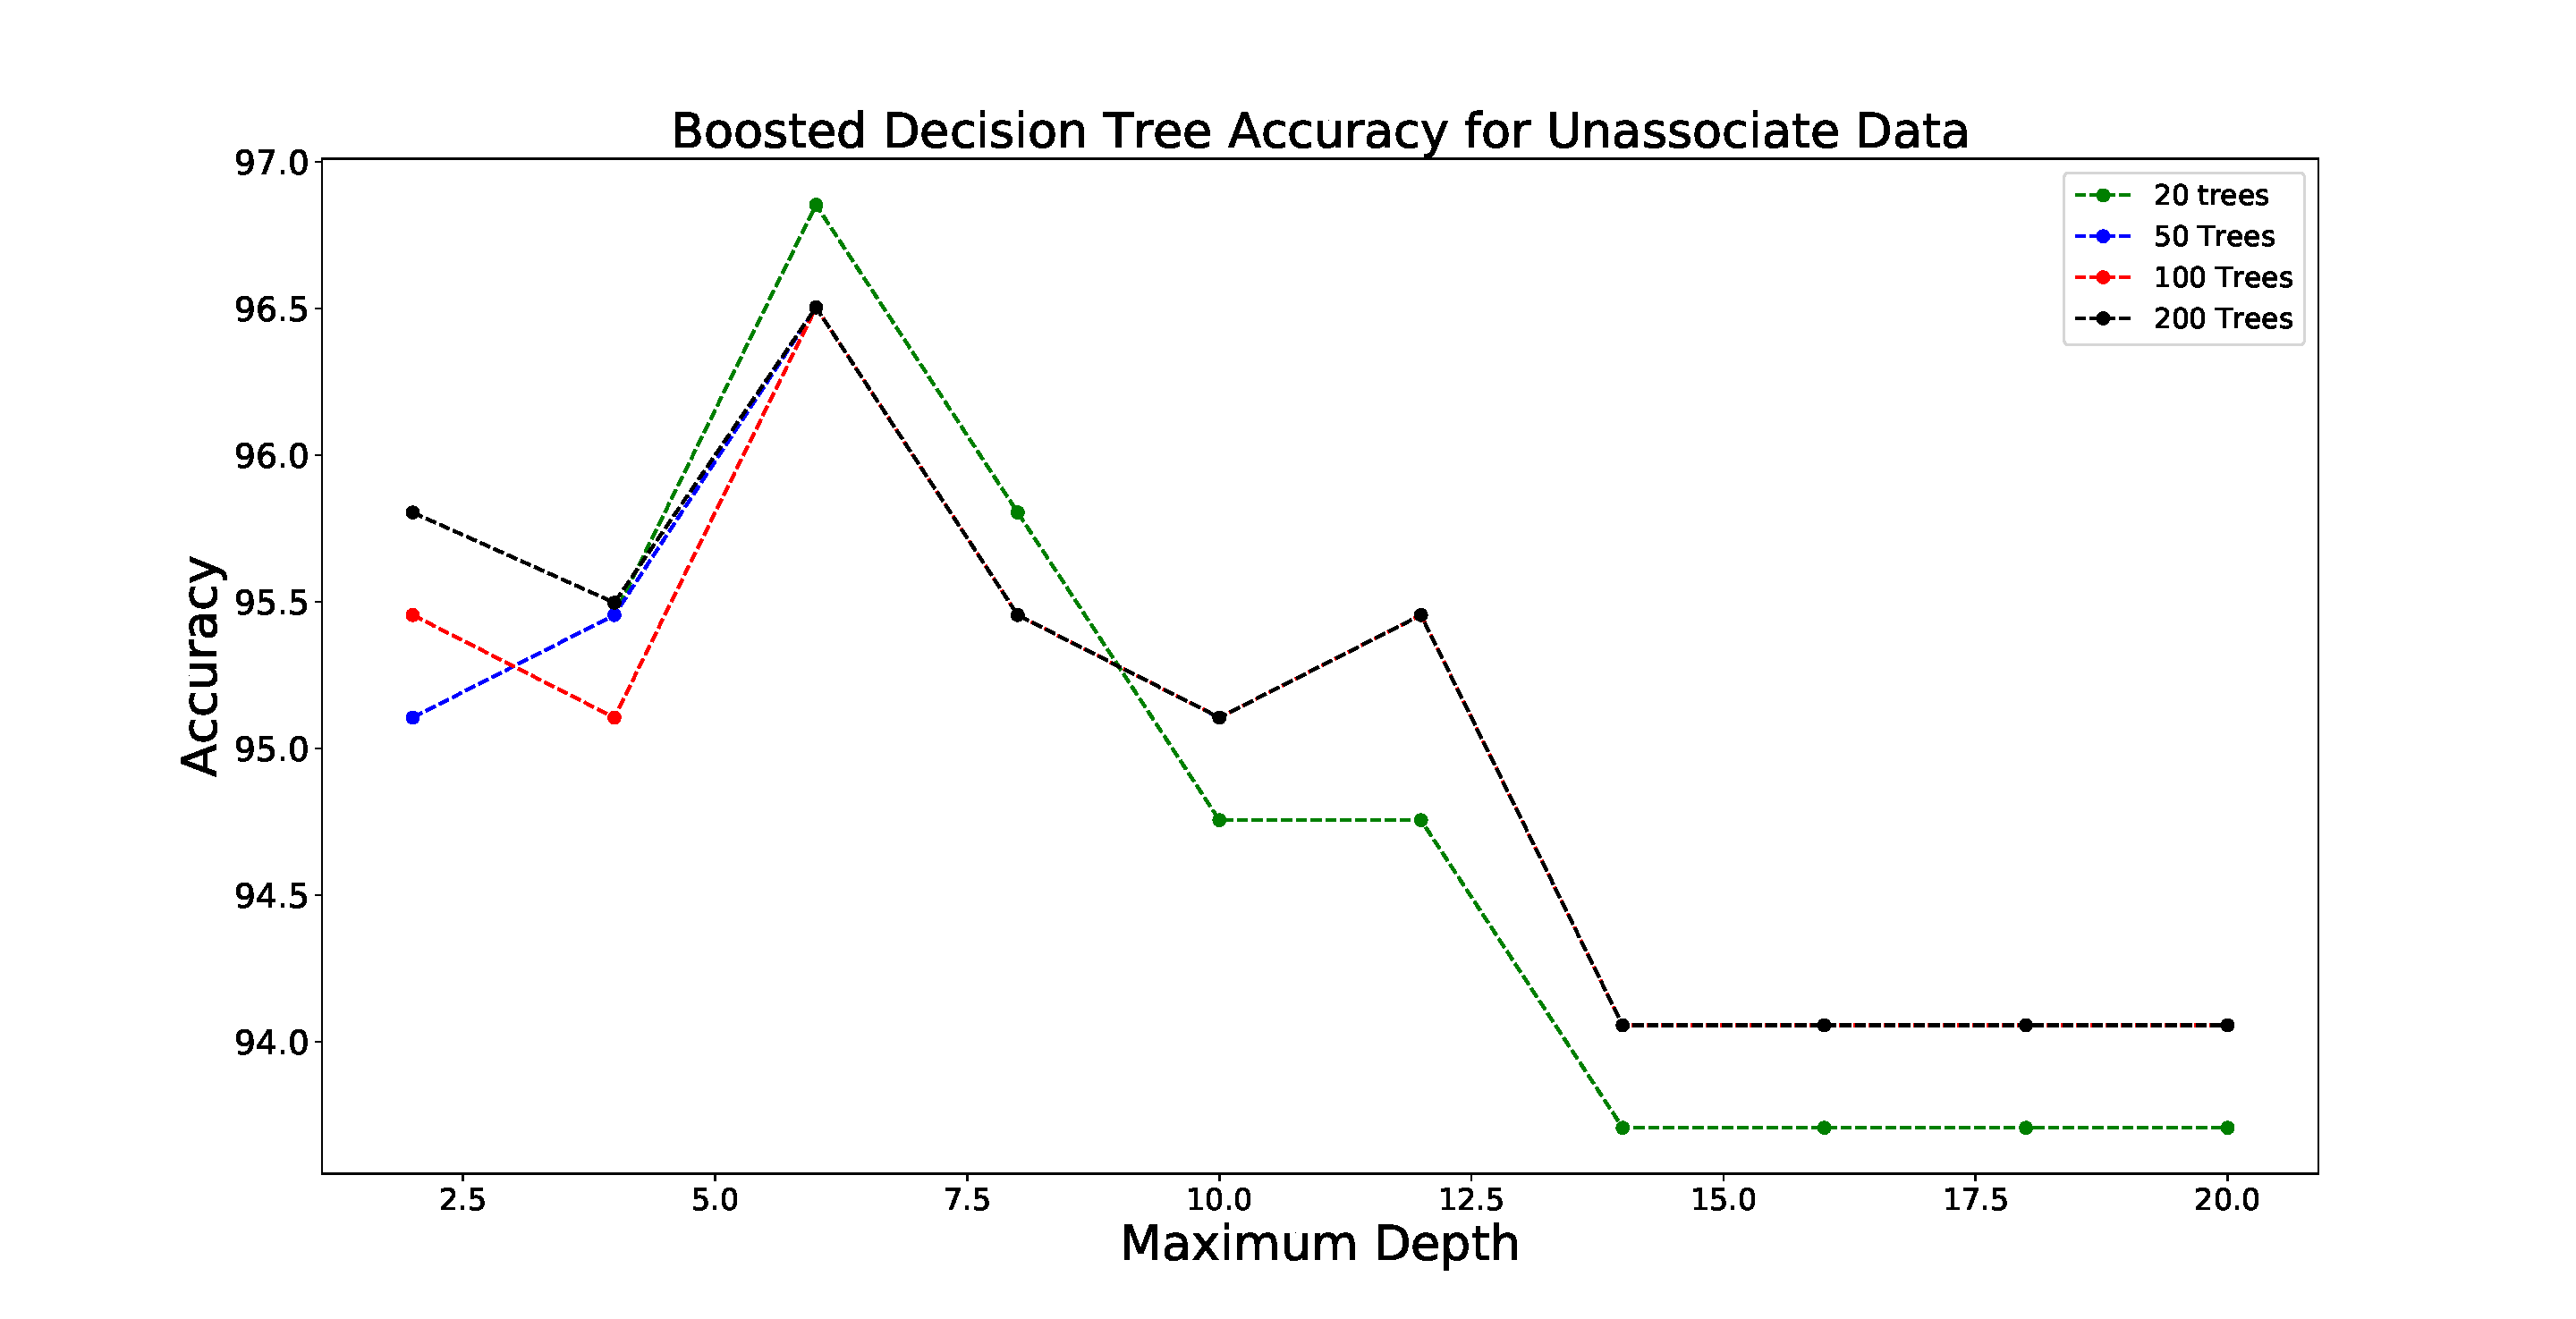
\includegraphics[width=\twopicsp\textwidth]{plots/unassoc_complex.pdf}
\caption{Random Forest and BDT accuracy on unassociated data as a function of complexity of the model}
\label{fig:Maps_data}
\end{figure}

Neural Networks, unlike random forests are susceptible to overtraining, as can be seen in the figures below. Increase the complexity of the network leads to a slight decrease in accuracy. This is seen for both single hidden layer networks and two hidden layer networks where the first layer has 5 neurons. Here Adam slightly outperforms lbfgs, especially when different activation functions are used. \\
An important result however is found for Logistic Regression case where the SAGA solver performs better than the normal lbfgs, reversing the trend seen in the training dataset. This is most likely because the SAGA solver allows for a more general model than the lbfgs one.\\
\begin{figure}[h]
%\centerin
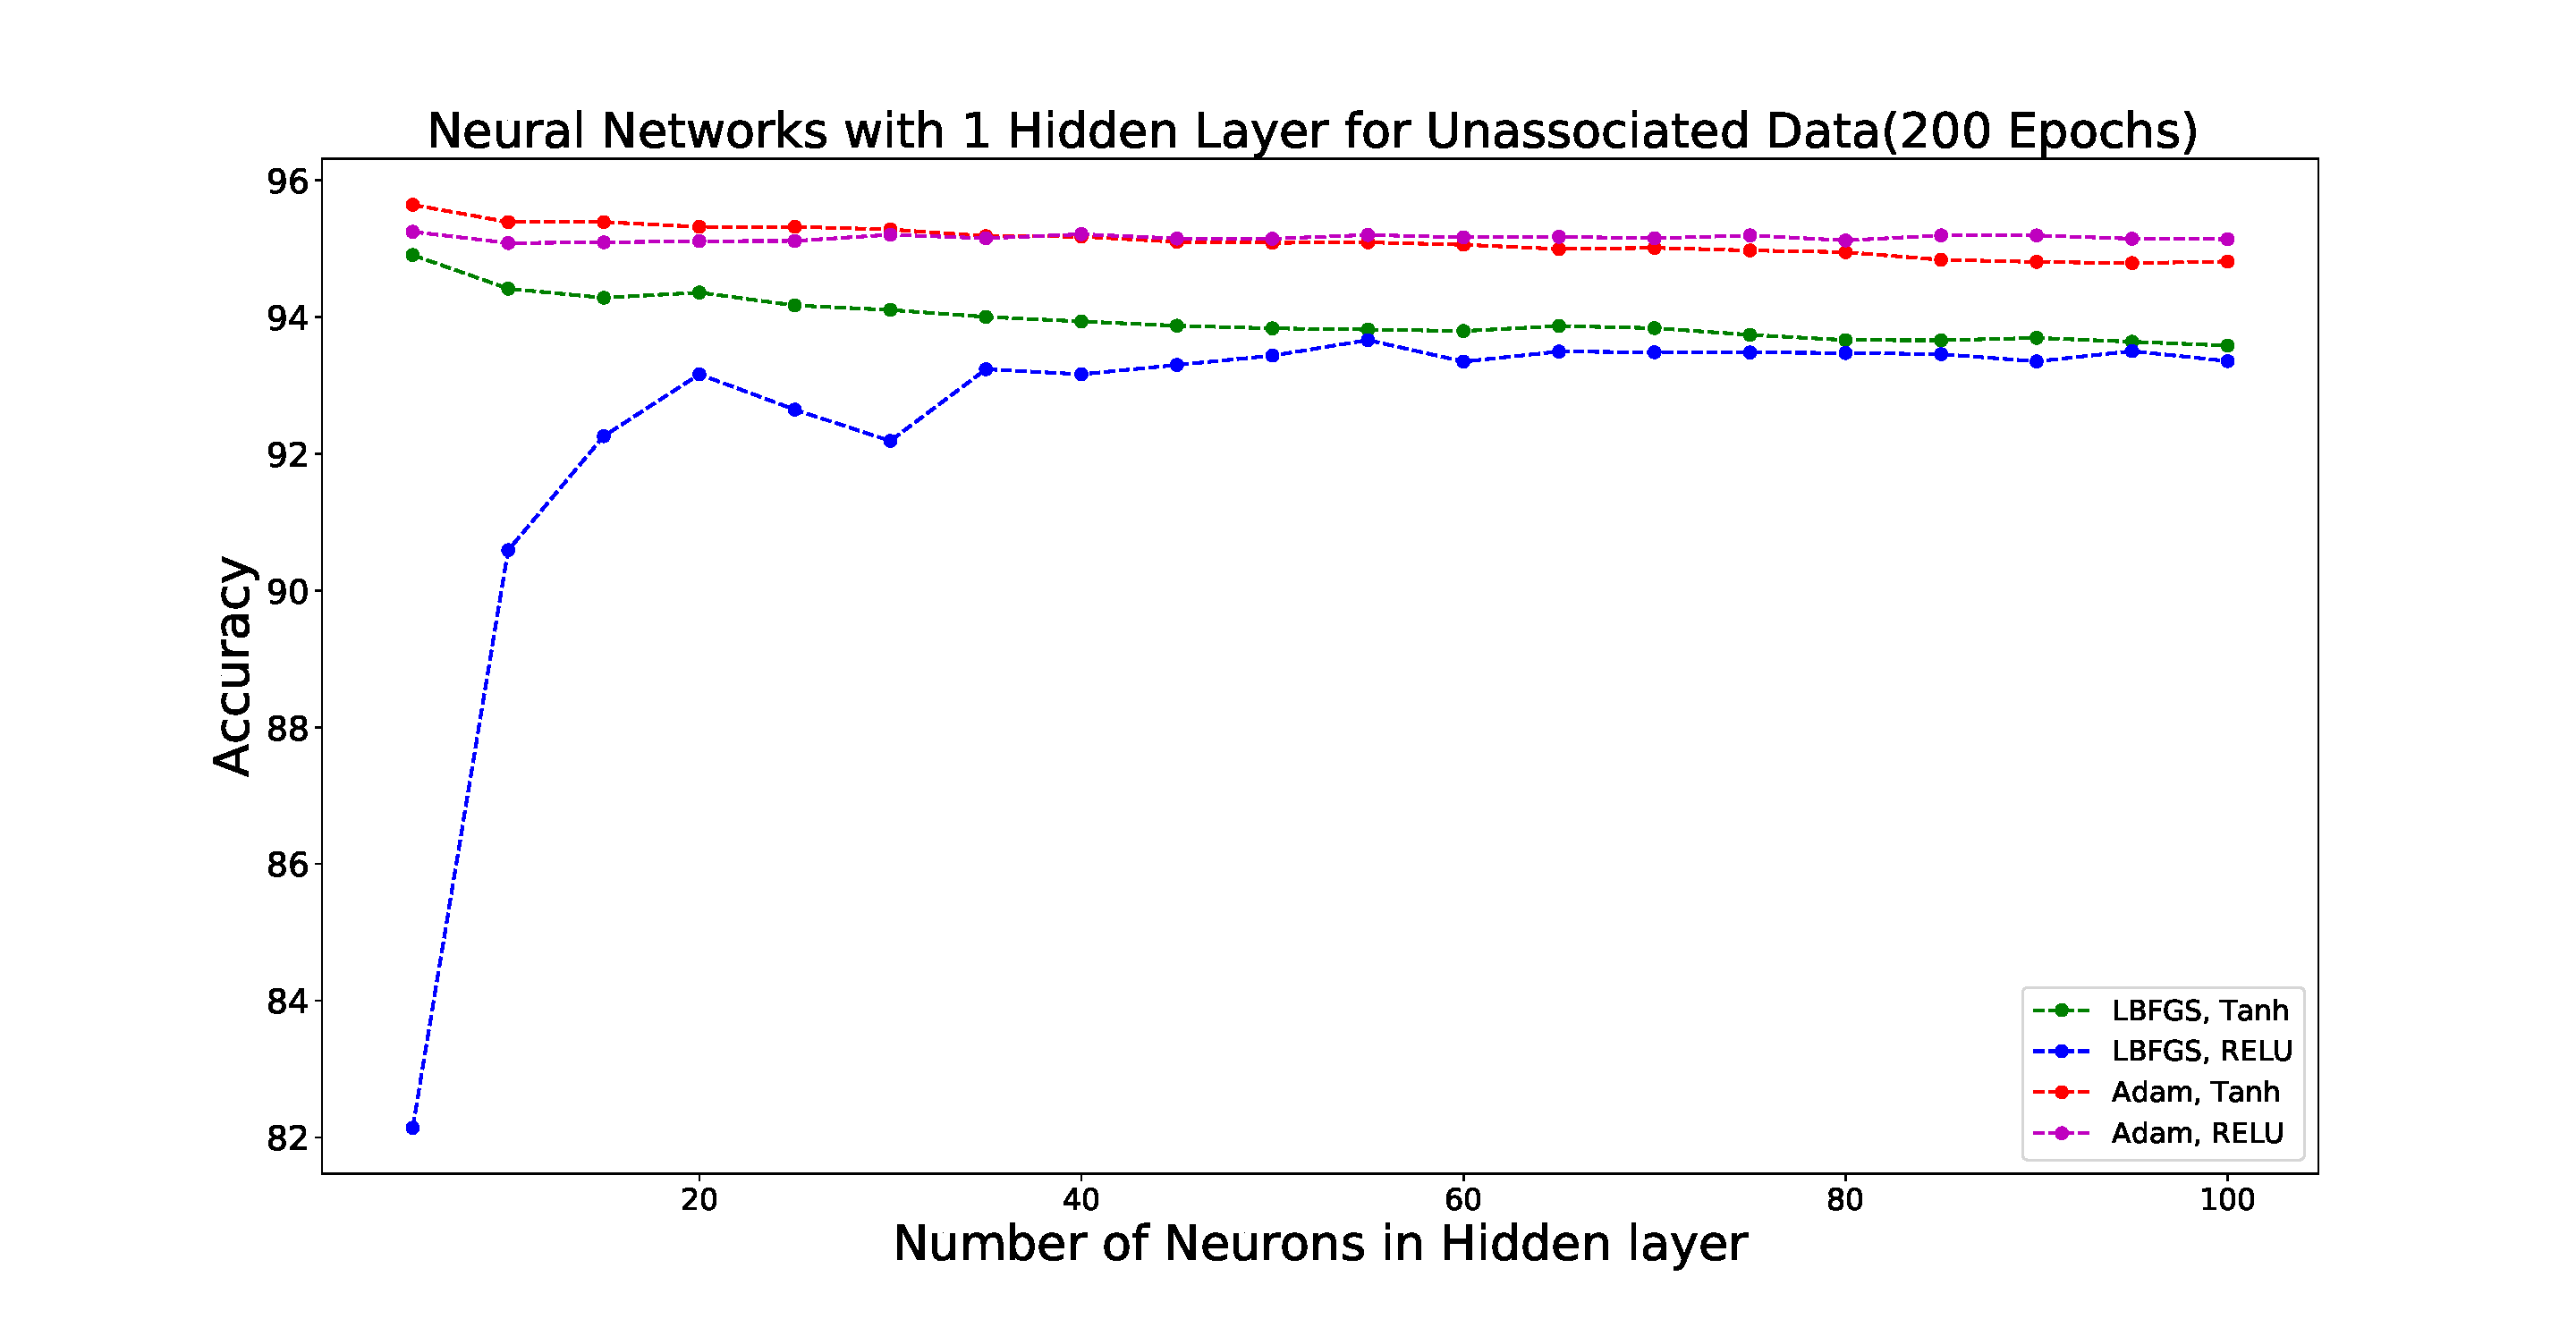
\includegraphics[width=\twopicsp\textwidth]{plots/neurons4.pdf}
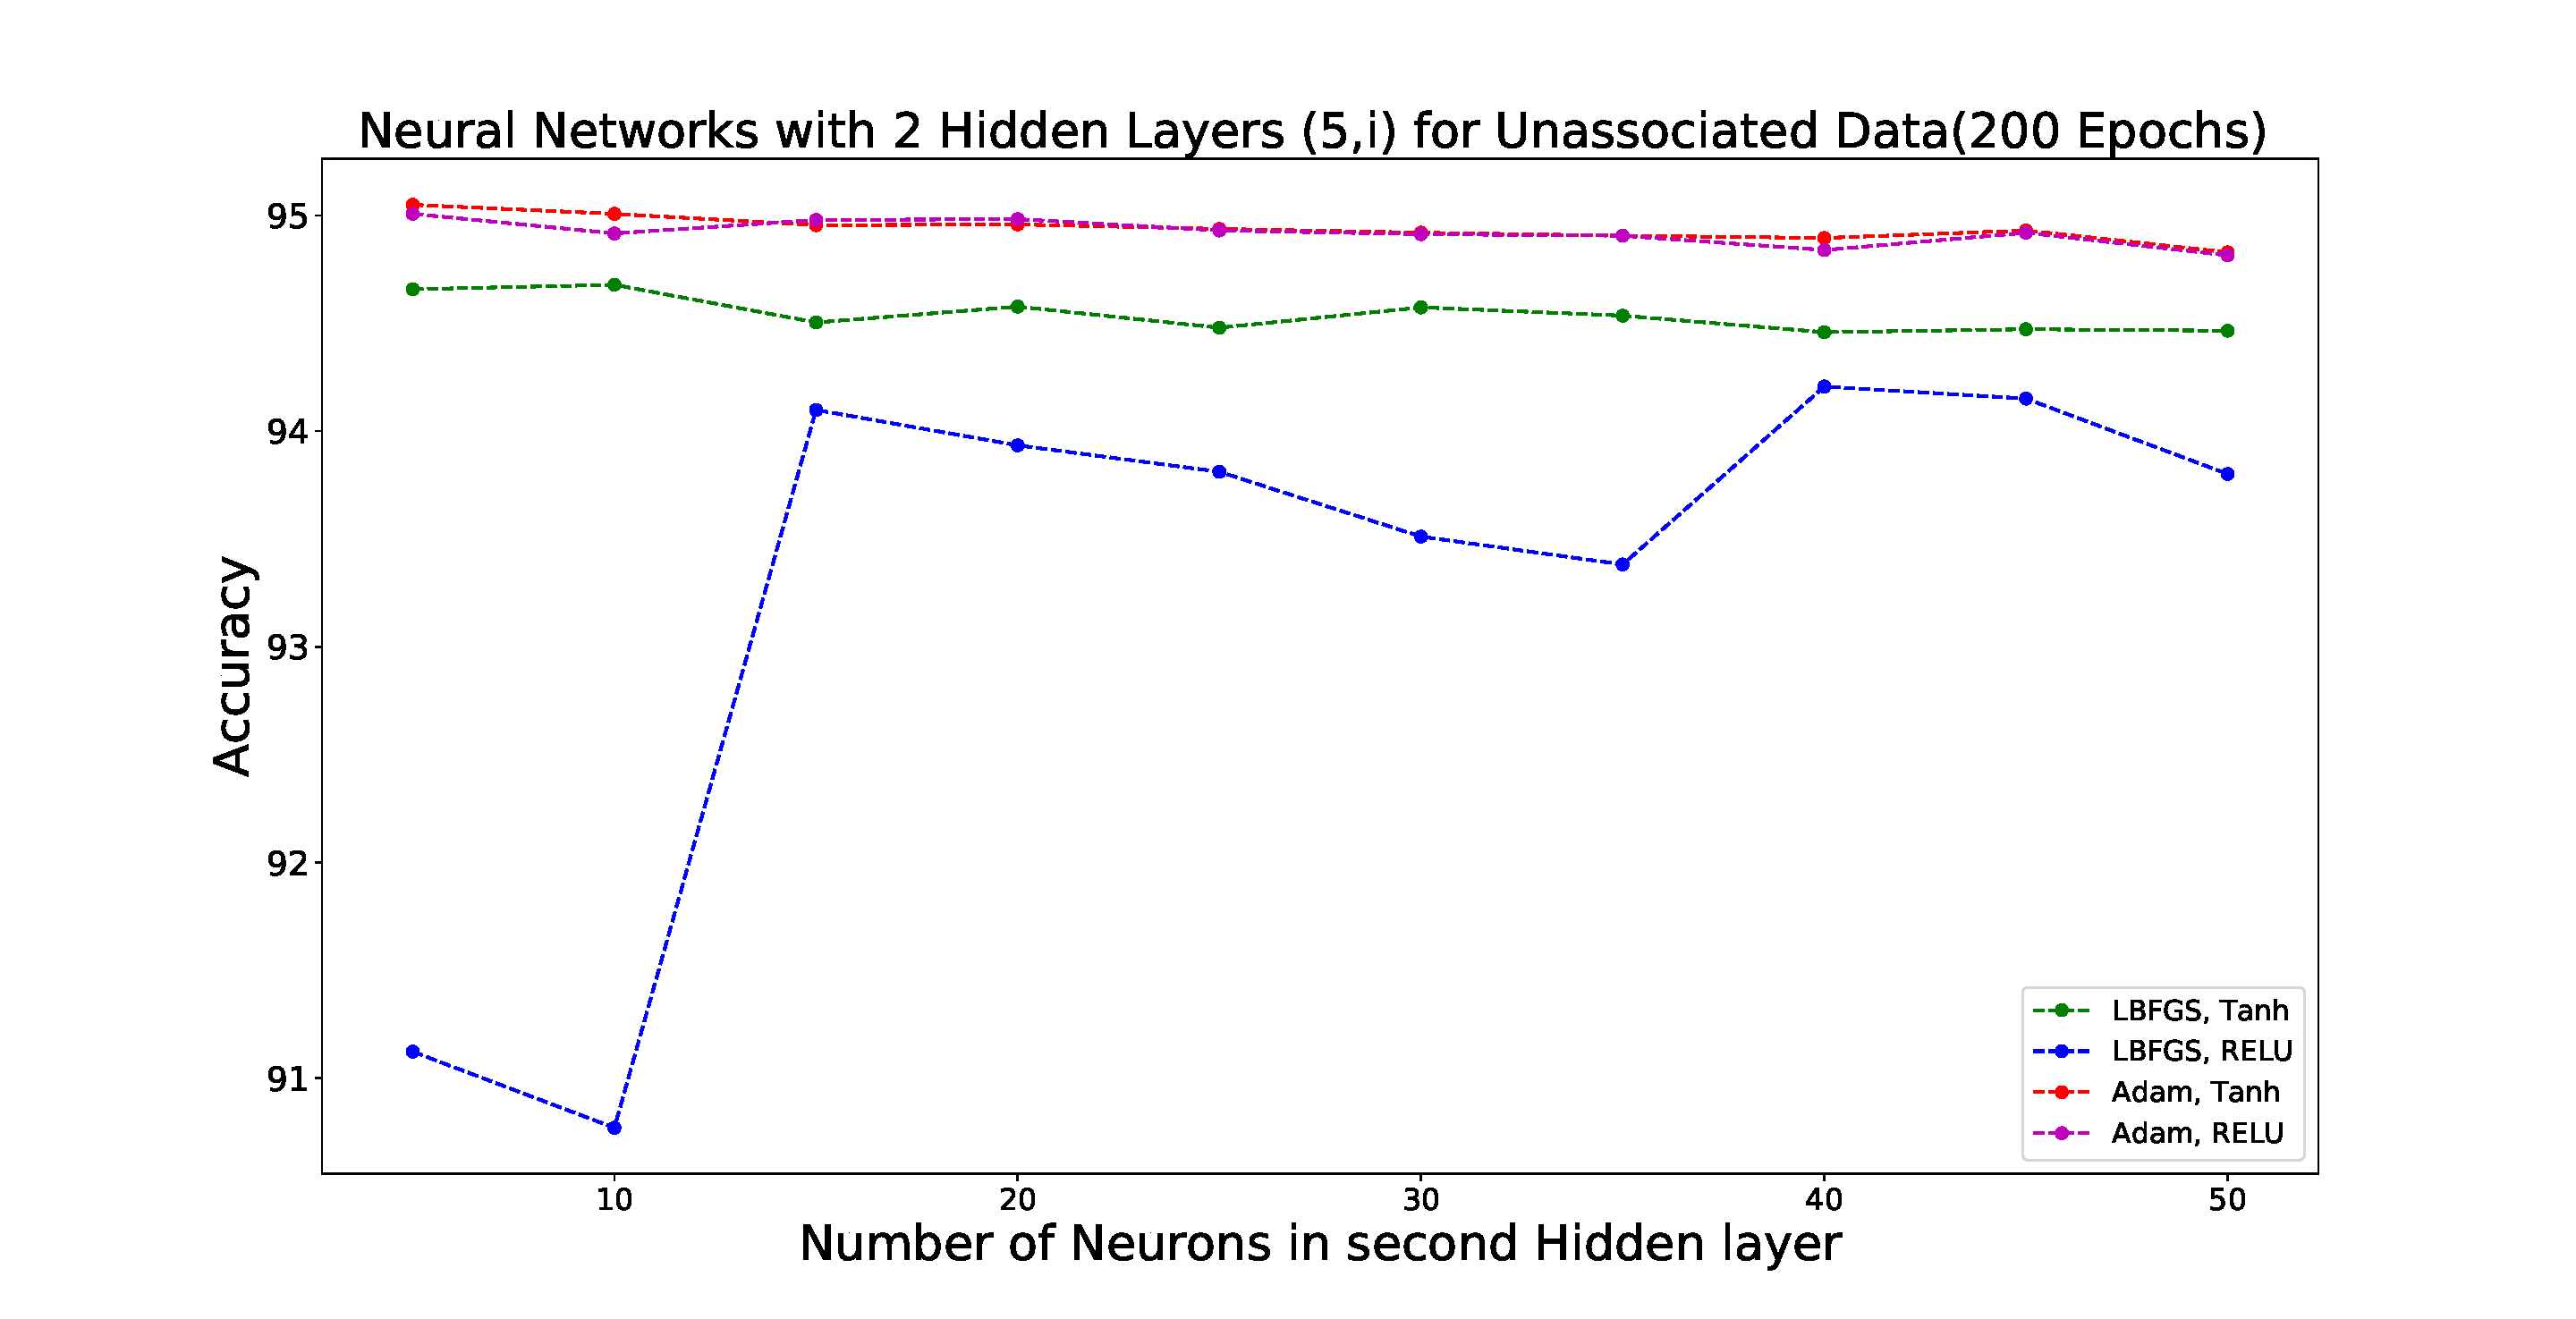
\includegraphics[width=\twopicsp\textwidth]{plots/neurons5.pdf}
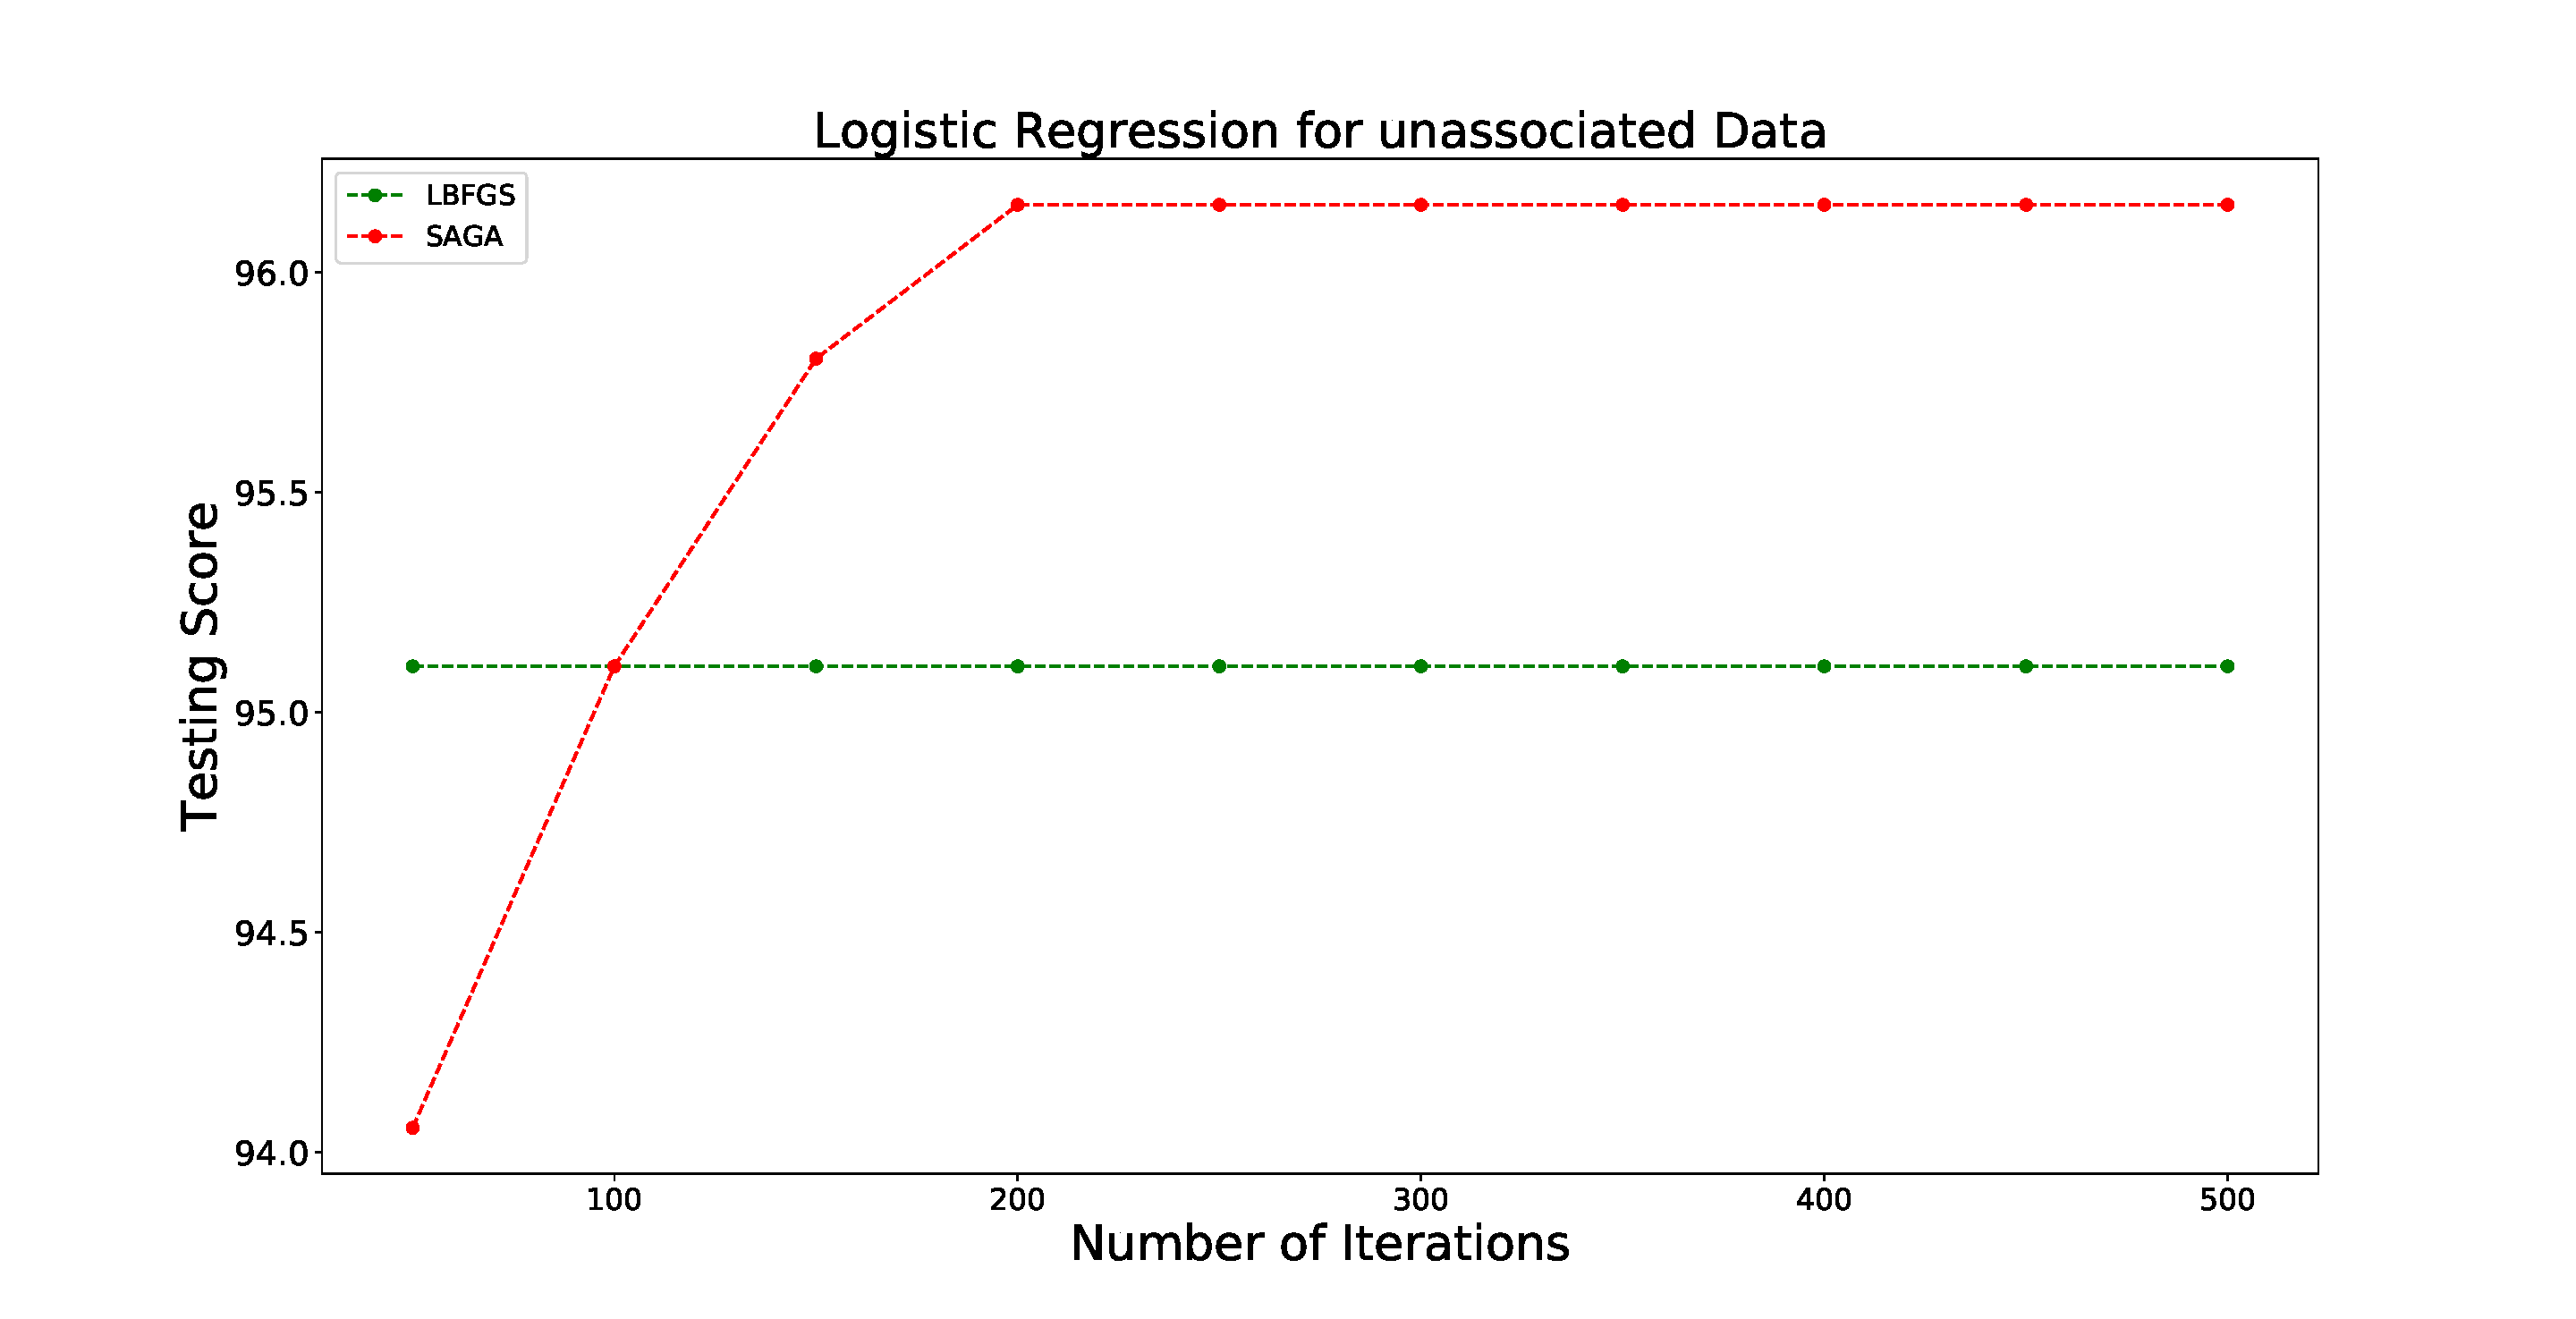
\includegraphics[width=\twopicsp\textwidth]{plots/solver_unass.pdf}
\caption{Logistic Regression and Neural Network accuracies}
\label{fig:Maps_data}
\end{figure}


 

Finally, we chose our best models to create a probabilistic catalog. The following were the accuracies we found for 1000 runs using the best models we had:\\



\begin{table}[!h]
    \tiny
    \centering
    \renewcommand{\tabcolsep}{1mm}
\renewcommand{\arraystretch}{1.5}

    \begin{tabular}{|c|c|c|}
    \hline
    Algorithm Name&Parameters & Accuracy\\
    \hline
    Random Forest& 200,15  & 96.55   \\
    \hline
    Neural Network & 200, ADAM, Tanh, 5 Neur     &  95.58 \\
    \hline %\midrule   -> aakash do you mean this?
    Gradient Boost& 50,10    &   95.27  \\
    \hline %\midrule   -> aakash do you mean this?
    Gradient Boost&200,2    &   95.8  \\
    \hline
    Logistic Regression& SAGA, 200 &95.45 \\
    \hline
     
    \end{tabular}

    \caption{Testing Accuracy of 4 algorithms on 3FGL unassociated data}
    \label{tab:my_labe2l}
\end{table}


As can be seen above, the best accuracies were found with less complicated models, which allowed bias to be low. The models were complicated enough to neither under, nor overtrain. \\

\subsection{3FGL Probabilistic classification} 

\begin{figure}[h]
%\centerin
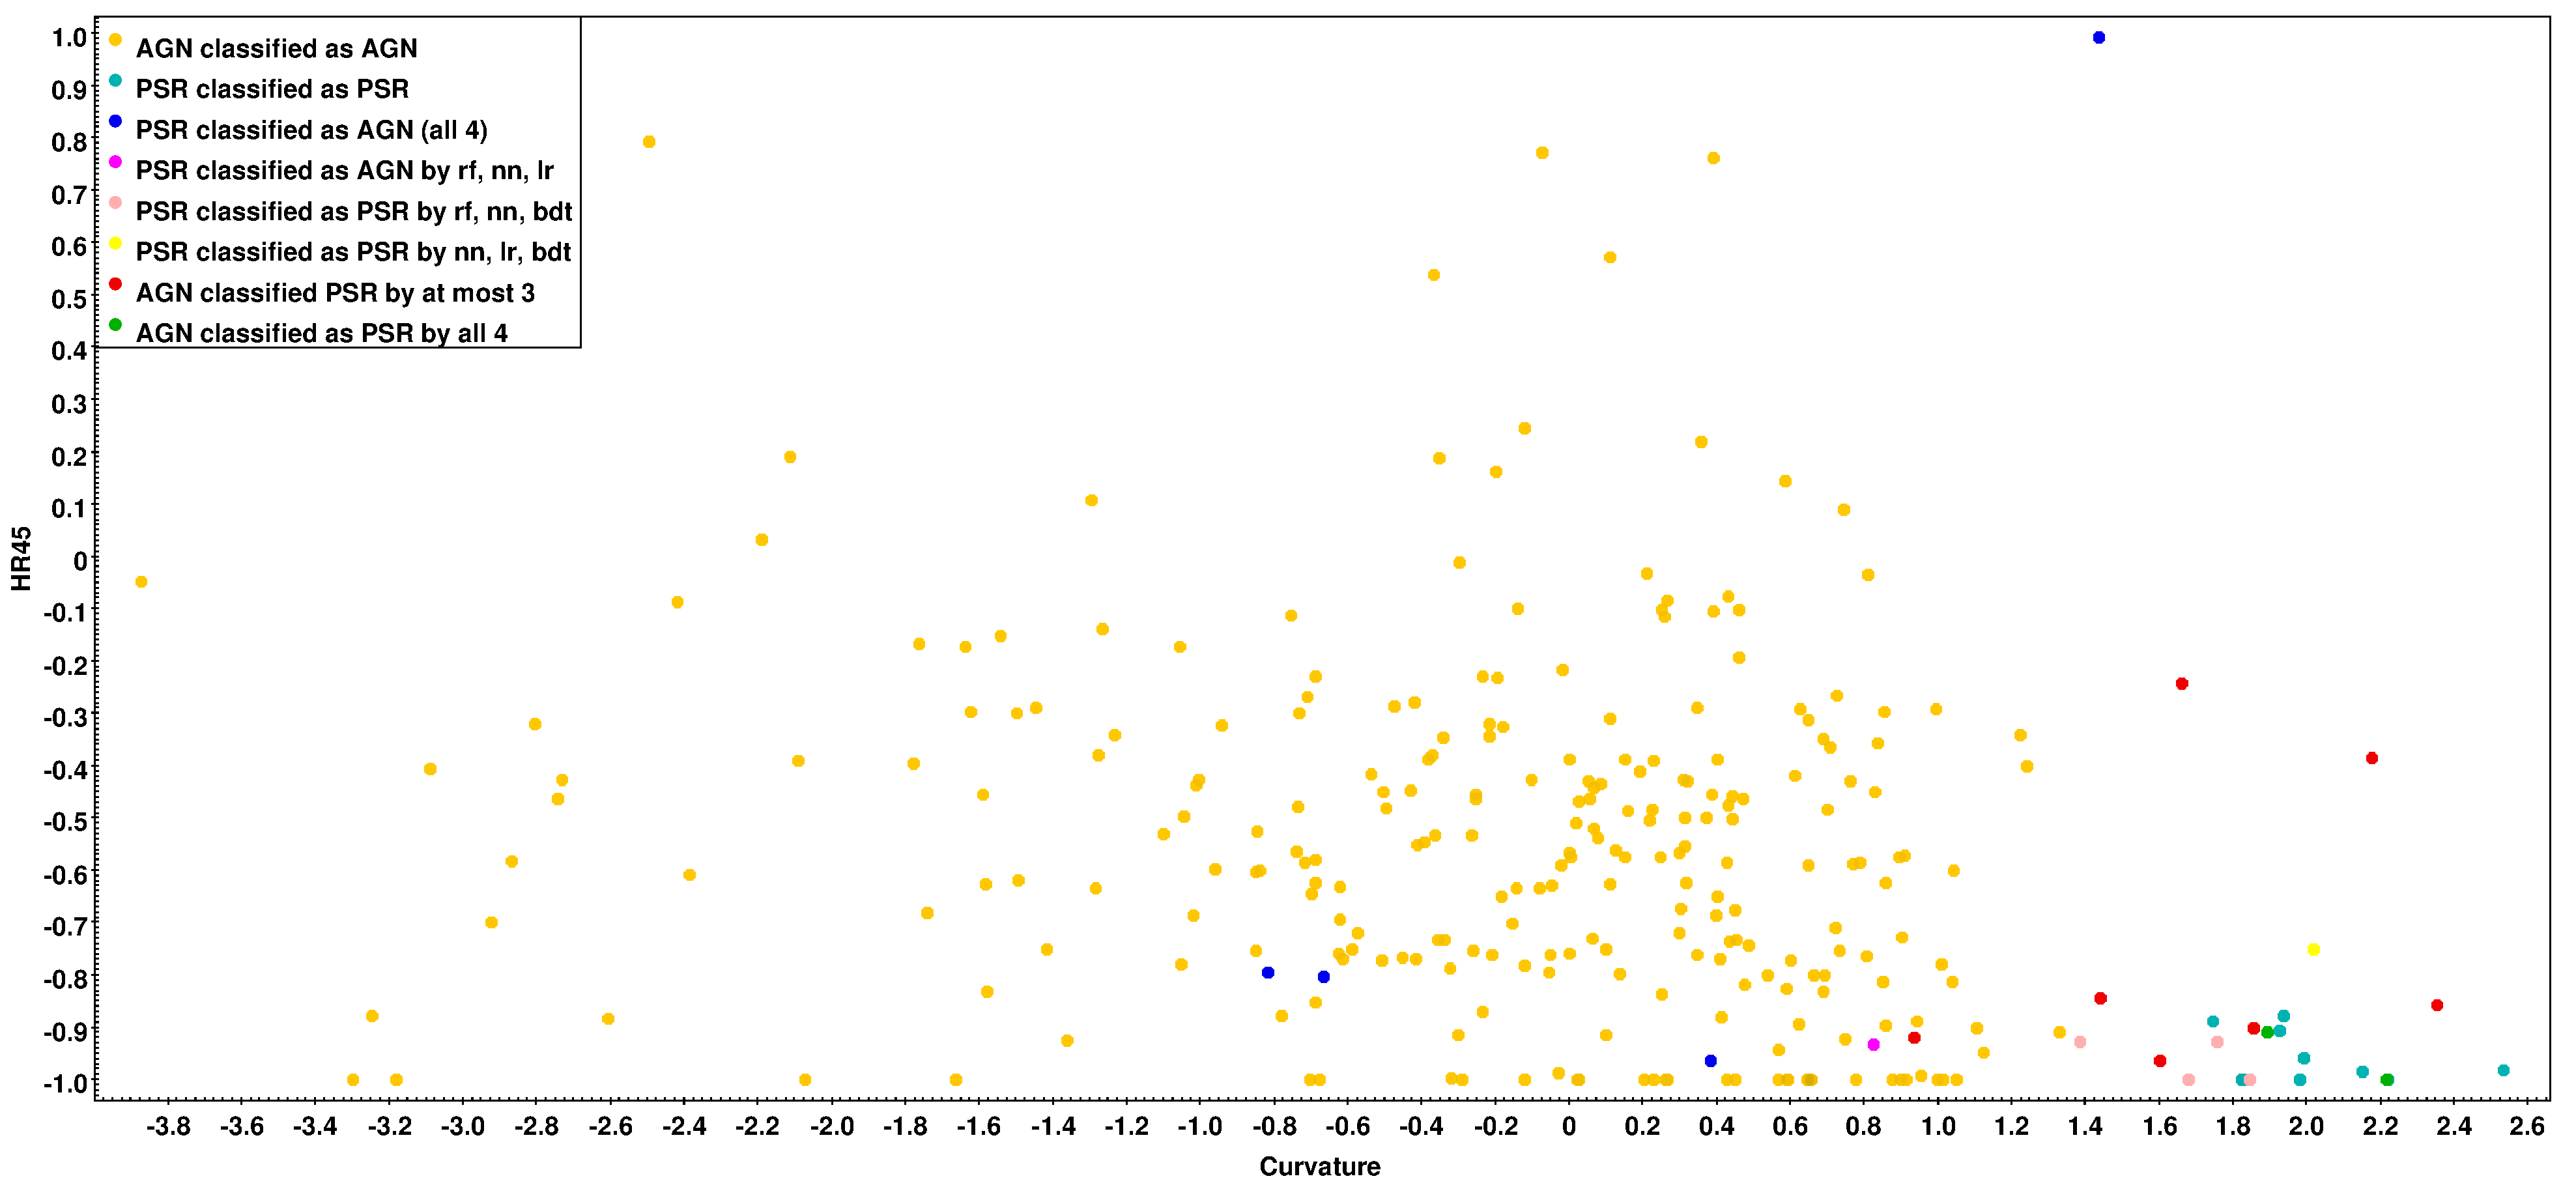
\includegraphics[width=\twopicsp\textwidth]{plots/final_catalog.pdf}
\caption{A comparison of the outliers in the test predictions}
\label{fig:Maps_data}
\end{figure}
